%% Compile: pdflatex > pdflatex
%% Final thesis presentation, built from thesisv4.tex and generated results tables.

\documentclass[aspectratio=169, 11pt]{beamer}

\usepackage[utf8]{inputenc}
\usepackage[T1]{fontenc}
\usepackage{textcomp}
\usepackage{lmodern}
\usepackage[british]{babel}

\usepackage{amsmath,amssymb}
\usepackage{booktabs}
\usepackage{array}
\usepackage{graphicx}
\usepackage{tikz}
\usetikzlibrary{positioning, arrows, calc, shapes.geometric,
  fit, backgrounds, decorations.pathreplacing, decorations.pathmorphing}
\usepackage{pgfpages}

\definecolor{Navy}{HTML}{0D1B2A}
\definecolor{MidNavy}{HTML}{1B2E4A}
\definecolor{DkOrange}{HTML}{D97706}
\definecolor{LtOrange}{HTML}{F5DEB3}
\definecolor{Bordeaux}{HTML}{7A1C2E}
\definecolor{BordeauxLt}{HTML}{A63D50}
\definecolor{Ivory}{HTML}{FAF8F5}
\definecolor{WarmGrey}{HTML}{E8E4DF}
\definecolor{MidGrey}{HTML}{9CA3AF}
\definecolor{DkGrey}{HTML}{4B5563}
\definecolor{Teal}{HTML}{2A7F8C}
\definecolor{TealLt}{HTML}{D0ECF0}
\definecolor{ForestGreen}{HTML}{4A7C59}
\definecolor{DeepRed}{HTML}{C44536}

\usefonttheme{professionalfonts}
\setbeamercolor{normal text}{fg=Navy, bg=Ivory}
\setbeamercolor{alerted text}{fg=Bordeaux}
\setbeamercolor{example text}{fg=DkOrange}

% Frame title
\setbeamercolor{frametitle}{fg=Ivory, bg=Navy}
\setbeamerfont{frametitle}{size=\large, series=\bfseries}
\setbeamertemplate{frametitle}{%
  \nointerlineskip
  \begin{beamercolorbox}[wd=\paperwidth, ht=2.6em, dp=0.8em, leftskip=1.2em]{frametitle}%
    \usebeamerfont{frametitle}\insertframetitle%
  \end{beamercolorbox}%
  {\color{DkOrange}\hrule height 2.2pt}%
}

% Title page
\setbeamercolor{title}{fg=Ivory}
\setbeamercolor{subtitle}{fg=LtOrange}
\setbeamercolor{author}{fg=Ivory}
\setbeamercolor{date}{fg=WarmGrey}
\setbeamercolor{institute}{fg=WarmGrey}
\setbeamerfont{title}{size=\Large, series=\bfseries}
\setbeamerfont{subtitle}{size=\normalsize, shape=\itshape}

% Itemize
\setbeamertemplate{itemize item}{\color{DkOrange}\scriptsize$\blacksquare$}
\setbeamertemplate{itemize subitem}{\color{Bordeaux}\scriptsize$\blacktriangleright$}
\setbeamercolor{itemize item}{fg=DkOrange}
\setbeamercolor{itemize subitem}{fg=Bordeaux}

% Footer
\setbeamertemplate{navigation symbols}{}
\setbeamertemplate{footline}{%
  \hfill
  \raisebox{3pt}{\color{MidGrey}\scriptsize\insertframenumber\,/\,\inserttotalframenumber}%
  \hspace{8pt}\vspace{3pt}%
}

% Blocks
\setbeamercolor{block title}{fg=Ivory, bg=MidNavy}
\setbeamercolor{block body}{fg=Navy, bg=WarmGrey}
\setbeamercolor{block title alerted}{fg=Ivory, bg=Bordeaux}
\setbeamercolor{block body alerted}{fg=Navy, bg=WarmGrey}
\setbeamercolor{block title example}{fg=Ivory, bg=DkOrange}
\setbeamercolor{block body example}{fg=Navy, bg=WarmGrey}
\setbeamerfont{block title}{series=\bfseries}

\AtBeginSection[]{}

\newcommand{\highlight}[1]{\textcolor{DkOrange}{\textbf{#1}}}
\newcommand{\emphbx}[1]{\textcolor{Bordeaux}{\textbf{#1}}}
\newcommand{\EUR}{\texteuro}
\newcommand{\USD}{US\$}
\newcommand{\pp}{\text{pp}}
\newcommand{\sourceline}[1]{}

\newcolumntype{L}[1]{>{\raggedright\arraybackslash}p{#1}}
\newcolumntype{C}[1]{>{\centering\arraybackslash}p{#1}}

\title{Decomposition of Global Minimum Tax Revenue\\Using CbCR Data}
\subtitle{An economic policy decomposition of measurement, behaviour and legal allocation}
\author{Maurits de Haan}
\institute{MSc Economic Policy, Utrecht University School of Economics}
\date{16 June 2026}

\begin{document}

{
\setbeamercolor{background canvas}{bg=Navy}
\begin{frame}[plain]
  \vspace{1.25em}
  \begin{center}
    {\color{Ivory}\Large\bfseries Decomposition of Global Minimum Tax Revenue}\\[0.25em]
    {\color{Ivory}\Large\bfseries using CbCR Data}\\[0.8em]
    {\color{DkOrange}\rule{6.4cm}{2pt}}\\[0.8em]
    {\color{LtOrange}\normalsize\itshape An economic policy decomposition of measurement, behaviour\\[0.15em]
     and legal allocation}\\[1.55em]
    {\color{Ivory}\normalsize Maurits de Haan}\\[0.3em]
    {\color{WarmGrey}\small MSc Economic Policy, Utrecht University}\\[0.25em]
    {\color{MidGrey}\small Final thesis presentation, 16 June 2026}
  \end{center}
\end{frame}
}

\section{Core argument}

\begin{frame}{Research question and empirical route}
\footnotesize
\textbf{Research question:} How much of the uncertainty in EU Global Minimum Tax revenue estimates is generated by measurement, substance, behaviour and collection rules?

\vspace{0.25em}
\begin{center}
\scriptsize
\setlength{\tabcolsep}{4pt}
\begin{tabular}{@{}C{0.85cm}L{2.75cm}L{6.85cm}@{}}
  \toprule
  & Short question & What is estimated \\
  \midrule
  SQ1 & Measure the base & Profit below the 15\% floor \\
  SQ2 & Add substance & Profit protected by payroll and tangible assets \\
  SQ3 & Add behaviour & Reported profit retained once the floor binds \\
  SQ4 & Allocate revenue & The treasury that can collect the residual top-up tax \\
  SQ5 & Read countries & Member States facing measurement, allocation or substance risk \\
  \bottomrule
\end{tabular}
\end{center}

\vspace{0.25em}
\centering
\emphbx{Design:} switch five modelling and policy choices on or off in one controlled 32-scenario revenue model, then decompose which choices move the forecast.
\end{frame}

\begin{frame}{Data used}
\small
\begin{center}
\scriptsize
\begin{tabular}{@{}L{3.35cm}L{4.15cm}L{3.85cm}@{}}
  \toprule
  Data source & What is observed & Use in the model \\
  \midrule
  OECD CbCR Table I & parent-affiliate profit, tax accrued, employees and tangible assets & corrected profit base, ETRs, activity proxies \\
  OECD CbCR Table IV & profit by subsidiary-level ETR bracket & direct 0 to 15\% low-taxed mass and validation \\
  OECD percentile ETR data & ETR percentiles where Table IV is absent or needs checking & distributional low-taxed share and gap \\
  FATS and EU KLEMS & sectoral payroll, turnover and tangible-capital structure & substance shield and SBTI capacity \\
  Fiscal and legal sources & CIT revenue, GDP, population, implementation status & fiscal salience and collector-country allocation \\
  \bottomrule
\end{tabular}
\end{center}

\vspace{0.3em}
\begin{block}{Scope}
  \footnotesize Data type: public aggregate country-by-country panel, not firm microdata. \\ Scope: 15,758 parent-affiliate-year cells, 58 parent and 228 affiliate jurisdictions, 2017 to 2022.
\end{block}
\end{frame}

\section{Measurement}

\begin{frame}{Measurement framework}
\footnotesize
\vspace{-0.15em}
\begin{block}{Three translations}
\scriptsize
\begin{columns}[T,totalwidth=\linewidth]
\begin{column}{0.31\linewidth}
\textcolor{DkOrange}{\textbf{1. Correct the base}}\\[0.15em]
Measured profit falls from \USD46.7 tn to \USD34.8 tn after removing double counting.
\end{column}
\begin{column}{0.31\linewidth}
\textcolor{DkOrange}{\textbf{2. Locate the low-tax slice}}\\[0.15em]
Use Table IV ETR brackets where observed and distributional evidence where public data are incomplete.
\end{column}
\begin{column}{0.31\linewidth}
\textcolor{DkOrange}{\textbf{3. Apply the top-up gap}}\\[0.15em]
Measure the distance to 15\% before substance, behaviour and allocation rules.
\end{column}
\end{columns}
\end{block}

\vspace{0.35em}
\begin{columns}[T,onlytextwidth]
\begin{column}{0.53\textwidth}
\begin{block}{EU27 sectoral shielding rate}
\scriptsize
\centering
\setlength{\tabcolsep}{5pt}
\renewcommand{\arraystretch}{1.12}
\begin{tabular}{@{}L{2.85cm}C{1.25cm}C{1.75cm}@{}}
  \toprule
  Scenario & Average & Distributional \\
  \midrule
  Before substance & 3.18\% & 5.17\% \\
  Initial SBIE & 3.00\% & 4.73\% \\
  Long-run SBIE & 3.07\% & 4.90\% \\
  \bottomrule
\end{tabular}
\renewcommand{\arraystretch}{1}
\end{block}
\end{column}

\begin{column}{0.43\textwidth}
\begin{exampleblock}{Average versus distributional ETR}
\scriptsize
\textbf{Average ETR} asks whether a jurisdiction is below 15\% on average.\\[0.45em]
\textbf{Distributional ETR} asks how much profit inside that jurisdiction is below 15\%.
\end{exampleblock}
\end{column}
\end{columns}
\end{frame}

\section{Behaviour}

\begin{frame}{Behavioural response: what is estimated}
\footnotesize
\begin{center}
\resizebox{0.92\linewidth}{!}{$\log \pi^{*}_{pjt}= \alpha_{pj}+\gamma_t+\beta_{\tau}\tau_{pjt}+\beta_A\log A_{pjt}+\beta_W\log \widehat{W}_{pjt}+X_{jt}'\delta+\varepsilon_{pjt}$}
\end{center}

\vspace{0.25em}
\begin{columns}[T]
\begin{column}{0.48\textwidth}
\begin{block}{Plain reading}
  Within the same parent-affiliate relationship, compare years with different ETRs while holding relationship and year effects fixed.
\end{block}
\begin{alertblock}{Use in the forecast}
  The coefficient reduces reported profit only in behavioural scenarios. It is a disciplined scenario input, not the main revenue-ranking result.
\end{alertblock}
\end{column}
\begin{column}{0.49\textwidth}
\begin{center}
\scriptsize
\setlength{\tabcolsep}{3.5pt}
\begin{tabular}{@{}L{2.55cm}L{3.05cm}@{}}
  \toprule
  Quantity & Interpretation \\
  \midrule
  Semi-elasticity 1.50 & one pp higher ETR, 1.50\% lower reported profit \\
  5\% to 15\% ETR & 13.9\% of profit reallocated \\
  10\% to 15\% ETR & 7.2\% of profit reallocated \\
  Revenue main effect & -\USD46.7 bn, 2017 to 2022 \\
  Variance share & 5.1\%, meaningful but not dominant \\
  \bottomrule
\end{tabular}
\end{center}

\end{column}
\end{columns}
\end{frame}

\begin{frame}{Behavioural regression output}
\small
\begin{center}
\scriptsize
\begin{tabular}{@{}lccc@{}}
  \toprule
  & Linear & Quadratic & Logarithmic \\
  \midrule
  ETR & -1.500*** (0.272) & -1.761* (0.909) & -0.943 (0.973) \\
  ETR squared & & 0.438 (1.262) & \\
  Log shifted ETR & & & -0.214 (0.415) \\
  Log tangible assets & -0.017 (0.015) & -0.017 (0.015) & -0.017 (0.015) \\
  Log payroll proxy & 0.023 (0.034) & 0.023 (0.034) & 0.023 (0.034) \\
  \midrule
  $N$ & 8,971 & 8,971 & 8,971 \\
  Parent-affiliate pairs & 1,936 & 1,936 & 1,936 \\
  BIC rank & 1 & 3 & 2 \\
  $\Delta$BIC & 0.00 & 7.54 & 5.40 \\
  \bottomrule
\end{tabular}
\end{center}
\tiny All models include parent-affiliate and year fixed effects. Standard errors are two-way clustered by parent and affiliate.
\sourceline{generated Table stage3\_regression\_table}
\end{frame}

\section{Substance and Allocation}

\begin{frame}{Substance result: 15\% is not the economic floor}
\small
\begin{center}
\scriptsize
\setlength{\tabcolsep}{7pt}
\begin{tabular}{@{}lrrr@{}}
  \toprule
  Group & Floor before SBTI (\%) & Floor after SBTI (\%) & Change (pp) \\
  \midrule
  EU27 weighted & 14.2 & 11.9 & -2.3 \\
  Germany & 13.9 & 10.7 & -3.2 \\
  France & 13.8 & 10.2 & -3.6 \\
  Netherlands & 14.5 & 13.6 & -0.9 \\
  Ireland & 14.7 & 13.7 & -1.0 \\
  Luxembourg & 14.2 & 13.7 & -0.4 \\
  \bottomrule
\end{tabular}
\end{center}

\vspace{0.45em}
\begin{block}{Policy reading}
  EU27 weighted: 10.4\% SBIE ratio and 3.7\% SBTI capacity. The relevant policy object is the effective floor after substance, before behaviour and allocation.
\end{block}
\end{frame}

\begin{frame}{Side-by-Side: EU27 collection example, 2022}
\small
\begin{center}
\scriptsize
\setlength{\tabcolsep}{4pt}
\begin{tabular}{@{}L{3.05cm}C{2.15cm}C{2.25cm}L{3.45cm}@{}}
  \toprule
  Channel & Universal (US\$ bn) & Side-by-Side (US\$ bn) & Interpretation \\
  \midrule
  Protected collection & 35.4 & 35.4 & source and EU parent rules remain available \\
  Residual enforcement backstop & 27.8 & 9.6 & exposed collection right is restricted \\
  \midrule
  Total EU collector revenue & 63.2 & 45.0 & \(\Delta = -18.3\) \\
  \bottomrule
\end{tabular}
\end{center}

\vspace{0.22em}
\begin{center}
\scriptsize
\begin{tabular}{@{}lrrrr@{}}
  \toprule
  Country example & Universal & Side-by-Side & Loss & Source-rule protected \\
  \midrule
  Germany & 11.0 & 7.8 & 3.2 & 58.8\% \\
  Netherlands & 11.2 & 9.1 & 2.0 & 83.1\% \\
  France & 6.1 & 3.4 & 2.7 & 40.9\% \\
  \bottomrule
\end{tabular}
\end{center}
\end{frame}

\section{Combined Results}

\begin{frame}{Revenue decomposition}
\footnotesize
\begin{block}{How to read this table}
  Main share is the 32-scenario variance explained by one channel. Effect is the average change in cumulative EU revenue. Interactions add 6.0\%, but the ranking still survives.
\end{block}

\vspace{0.1em}
\begin{center}
\scriptsize
\begin{tabular}{@{}L{2.55cm}C{1.85cm}C{2.05cm}L{4.55cm}@{}}
  \toprule
  Channel & Main share (\%) & Effect (US\$ bn) & Economic interpretation \\
  \midrule
  Low-taxed base measurement & 69.1 & +197.0 & the public data must identify the low-taxed mass inside jurisdictions \\
  Collection-right rules & 15.0 & -87.5 & legal rules change where the revenue accrues \\
  Behaviour & 5.1 & -46.7 & firms respond, but this is not the main forecast driver \\
  Substance shield & 4.6 & -43.6 & payroll and tangible assets reduce the effective floor \\
  Rate endpoint & 0.1 & +8.6 & transition rates matter little in the full design \\
  \bottomrule
\end{tabular}
\end{center}

\end{frame}

\begin{frame}{Country policy readings}
\small
\begin{center}
\scriptsize
\setlength{\tabcolsep}{3pt}
\begin{tabular}{@{}L{1.65cm}r r r r L{2.6cm}@{}}
  \toprule
  Country & Rev. & Rev./CIT & Spread/CIT & QDMTT & Dominant channel \\
  \midrule
  Germany & 44.5 & 9.0 & 16.2 & 55.4 & ETR (84.1\%) \\
  Netherlands & 87.1 & 41.4 & 38.5 & 92.2 & ETR (72.9\%) \\
  France & 20.2 & 5.4 & 12.6 & 58.5 & ETR (72.7\%) \\
  Luxembourg & 51.7 & 225.1 & 181.7 & 92.6 & SbS (58.0\%) \\
  Ireland & 27.1 & 30.3 & 29.7 & 86.0 & substance (38.1\%) \\
  Hungary & 3.9 & 26.8 & 40.2 & 88.0 & ETR (54.9\%) \\
  \bottomrule
\end{tabular}
\end{center}

\vspace{0.3em}
\begin{alertblock}{Policy reading}
  Dominant channel is the largest country-level main effect in the 32-scenario spread. Read each row in order: fiscal salience (Rev./CIT), uncertainty (Spread/CIT), protected domestic collection (QDMTT), then the channel that moves the forecast range most.
\end{alertblock}
\end{frame}

\begin{frame}{Policy next steps}
\footnotesize
\begin{columns}[T]
\begin{column}{0.48\textwidth}
\begin{block}{1. Measure the base}
  Require bracket-level ETR reporting below 15\%. This directly targets the largest forecast driver.
\end{block}
\end{column}
\begin{column}{0.48\textwidth}
\begin{exampleblock}{2. Secure collection rights}
  Track QDMTT status and residual IIR/UTPR exposure. SbS changes who can collect, not where the low-taxed profit sits.
\end{exampleblock}
\end{column}
\end{columns}

\vspace{0.35em}
\begin{columns}[T]
\begin{column}{0.48\textwidth}
\begin{block}{3. Publish ranges}
  Report scenario decompositions beside the budget number. The 32-scenario range is economically material.
\end{block}
\end{column}
\begin{column}{0.48\textwidth}
\begin{alertblock}{4. Validate ex post}
  Reconcile forecasts with observed GloBE, QDMTT, SBIE and incentive-claim data once implementation data exist.
\end{alertblock}
\end{column}
\end{columns}

\vspace{0.45em}
\begin{block}{Policy implication}
  Priority order follows the decomposition: distributional measurement first, legal collection-right modelling second, then behavioural and substance validation.
\end{block}
\end{frame}

\begin{frame}{Conclusion}
\small
\begin{center}
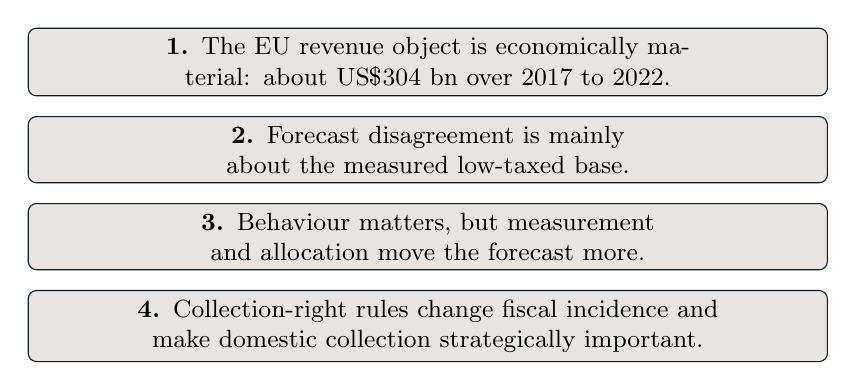
\begin{tikzpicture}[font=\small, node distance=0.38cm]
  \tikzset{
    point/.style={draw=Navy, rounded corners=3pt, fill=WarmGrey,
      minimum width=10.15cm, text width=9.55cm, minimum height=0.70cm, align=center}
  }
  \node[point] (p1) {\textbf{1.} The EU revenue object is economically material: about \USD304 bn over 2017 to 2022.};
  \node[point, below=0.25cm of p1] (p2) {\textbf{2.} Forecast disagreement is mainly about the measured low-taxed base.};
  \node[point, below=0.25cm of p2] (p3) {\textbf{3.} Behaviour matters, but measurement and allocation move the forecast more.};
  \node[point, below=0.25cm of p3] (p4) {\textbf{4.} Collection-right rules change fiscal incidence and make domestic collection strategically important.};
\end{tikzpicture}
\end{center}

\vspace{0.45em}
\centering
\highlight{The thesis contributes an economic policy decomposition of a contested fiscal forecast.}
\end{frame}

{
\setbeamercolor{background canvas}{bg=Navy}
\begin{frame}[plain]
  \vspace{1.45em}
  \begin{center}
    {\color{Ivory}\Large\bfseries Thank you}\\[1.15em]
    {\color{DkOrange}\rule{4.2cm}{2pt}}\\[1.15em]
    {\color{WarmGrey}\normalsize Measurement defines the base.}\\[0.38em]
    {\color{LtOrange}\normalsize Behaviour calibrates the response.}\\[0.38em]
    {\color{WarmGrey}\normalsize Collection rights determine fiscal incidence.}\\[1.25em]
    {\color{MidGrey}\small Maurits de Haan $\cdot$ m.c.p.dehaan@students.uu.nl}
  \end{center}
\end{frame}
}

\appendix

{
\setbeamercolor{background canvas}{bg=MidNavy}
\begin{frame}[plain]
  \vfill
  \centering
  {\color{Ivory}\LARGE\bfseries Backup slides}\\[0.6em]
  {\color{DkOrange}\rule{4cm}{2pt}}\\[0.8em]
  \vfill
\end{frame}
}

\begin{frame}{Backup: stronger measurement windows}
\small
\begin{center}
\scriptsize
\setlength{\tabcolsep}{3.5pt}
\begin{tabular}{@{}L{3.35cm}rrrrL{2.6cm}@{}}
  \toprule
  Sample window & ETR (\%) & Allocation (\%) & Substance (\%) & Behaviour (\%) & Revenue range (US\$ bn) \\
  \midrule
  2017 to 2022 public panel & 72.0 & 16.6 & 5.7 & 5.5 & 127.7 to 517.4 \\
  2019 to 2022 stronger measurement & 80.3 & 11.4 & 4.5 & 3.7 & 73.0 to 332.4 \\
  2021 to 2022 strict overlap & 84.5 & 9.2 & 3.9 & 2.2 & 32.1 to 175.3 \\
  \bottomrule
\end{tabular}
\end{center}

\vspace{0.55em}
\begin{block}{Reading}
  When the window relies more directly on ETR-bracket evidence, measurement becomes an even larger share of the forecast spread. Preferred revenues are US\$303.7 bn, US\$193.0 bn and US\$102.3 bn respectively.
\end{block}
\end{frame}

\begin{frame}{Backup: acronyms and collection rule}
\small
\begin{center}
\scriptsize
\begin{tabular}{@{}L{2.25cm}L{4.25cm}L{4.8cm}@{}}
  \toprule
  \textbf{Term} & \textbf{Plain meaning} & \textbf{Revenue role} \\
  \midrule
  QDMTT & qualified domestic minimum top-up tax & source country collects first \\
  IIR & income inclusion rule & parent country collects if source country does not \\
  UTPR & undertaxed profits rule & implementing countries collect residual backstop revenue \\
  Side-by-Side & safe harbour for qualifying parent regimes in the thesis model & residual IIR and UTPR set to zero for qualifying US-parented groups \\
  SBIE & substance-based income exclusion & payroll and tangible assets shield part of the base \\
  SBTI & substance-based tax incentive safe harbour & capacity for substance-linked incentives to be protected \\
  \bottomrule
\end{tabular}
\end{center}
\sourceline{thesisv4 Sections 3 and 4}
\end{frame}

\begin{frame}{Backup: source hierarchy for Stage 1}
\small
\begin{center}
\scriptsize
\begin{tabular}{@{}lrrrrrrr@{}}
  \toprule
  Source & 2017 & 2018 & 2019 & 2020 & 2021 & 2022 & Total \\
  \midrule
  Direct Table IV & 0 & 0 & 2,275 & 2,306 & 2,470 & 2,344 & 9,395 \\
  Beta percentile fit & 0 & 0 & 0 & 0 & 421 & 399 & 820 \\
  BSPI shape transport & 1,720 & 2,179 & 0 & 0 & 0 & 0 & 3,899 \\
  Jurisdiction-average fallback & 303 & 348 & 393 & 408 & 5 & 2 & 1,459 \\
  Missing source & 22 & 27 & 43 & 36 & 25 & 32 & 185 \\
  \bottomrule
\end{tabular}
\end{center}
\begin{block}{Interpretation}
  Direct Table IV carries the main distributional branch after 2019. The early years require shape transport, which is why the robustness slides restrict the window.
\end{block}
\sourceline{generated Table stage1\_source\_coverage}
\end{frame}

\begin{frame}{Backup: profit-base correction}
\small
\begin{columns}[T]
\begin{column}{0.48\textwidth}
\begin{center}
\scriptsize
\begin{tabular}{@{}lrr@{}}
  \toprule
  Profit branch & Reported & Corrected \\
  \midrule
  OECD adjusted & 851.0 & 609.2 \\
  External-anchor domestic & 5,308.8 & 2,491.1 \\
  Domestic model & 24,642.7 & 15,831.7 \\
  Foreign affiliates & 15,908.8 & 15,908.8 \\
  \midrule
  Total & 46,711.2 & 34,840.8 \\
  \bottomrule
\end{tabular}
\end{center}
\tiny Current US\$ bn.
\end{column}
\begin{column}{0.48\textwidth}
\begin{block}{Why it matters}
  The correction addresses double-counting exposure in domestic parent cells. It reduces positive-profit CbCR profit by 25.4\% before any GMT revenue stage is estimated.
\end{block}
\begin{alertblock}{Interpretive boundary}
  This is a denominator correction, not a claim about new tax payments.
\end{alertblock}
\end{column}
\end{columns}
\sourceline{generated Table profit\_correction\_effects}
\end{frame}

\begin{frame}{Backup: annual Stage 1 rates}
\small
\begin{center}
\scriptsize
\begin{tabular}{@{}lrrrrrr@{}}
  \toprule
  EU27 & 2017 & 2018 & 2019 & 2020 & 2021 & 2022 \\
  \midrule
  Average rule, low-taxed share & 53.9 & 63.3 & 62.5 & 55.0 & 55.3 & 41.8 \\
  Average rule, liability rate & 3.5 & 4.6 & 3.8 & 2.9 & 2.9 & 1.4 \\
  Distributional rule, low-taxed share & 52.3 & 55.6 & 53.4 & 50.9 & 51.5 & 43.8 \\
  Distributional rule, liability rate & 5.8 & 6.1 & 5.7 & 4.8 & 4.9 & 3.7 \\
  \bottomrule
\end{tabular}
\end{center}
\begin{block}{Reading}
  The distributional branch usually does not raise the low-taxed share dramatically. It raises the liability rate because the identified low-taxed slice has a larger average top-up gap.
\end{block}
\sourceline{generated Table stage1\_rates}
\end{frame}

\begin{frame}{Backup: behavioural regression output}
\small
\begin{center}
\scriptsize
\begin{tabular}{@{}lccc@{}}
  \toprule
  & Linear & Quadratic & Logarithmic \\
  \midrule
  ETR & -1.500*** (0.272) & -1.761* (0.909) & -0.943 (0.973) \\
  ETR squared & & 0.438 (1.262) & \\
  Log shifted ETR & & & -0.214 (0.415) \\
  Log tangible assets & -0.017 (0.015) & -0.017 (0.015) & -0.017 (0.015) \\
  Log payroll proxy & 0.023 (0.034) & 0.023 (0.034) & 0.023 (0.034) \\
  \midrule
  $N$ & 8,971 & 8,971 & 8,971 \\
  Parent-affiliate pairs & 1,936 & 1,936 & 1,936 \\
  BIC rank & 1 & 3 & 2 \\
  $\Delta$BIC & 0.00 & 7.54 & 5.40 \\
  \bottomrule
\end{tabular}
\end{center}
\tiny All models include parent-affiliate and year fixed effects. Standard errors are two-way clustered by parent and affiliate.
\sourceline{generated Table stage3\_regression\_table}
\end{frame}

\begin{frame}{Backup: behavioural reliability scorecard}
\small
\begin{center}
\scriptsize
\begin{tabular}{@{}L{3.3cm}L{4.2cm}L{4.2cm}@{}}
  \toprule
  Diagnostic & Result & Weight for interpretation \\
  \midrule
  Preferred FE estimate & semi-elasticity 1.50; $N=8,971$; pairs $=1,936$ & usable scenario coefficient \\
  Model selection & BIC selects linear; tax Wald $p=1.5\times10^{-6}$ & supports parsimonious response \\
  Two-way inference & SE $=0.272$; $p=1.5\times10^{-6}$ & statistically strong association \\
  IV diagnostics & first stages relevant; 2SLS imprecise & weak for causal replacement \\
  Low-ETR tail & below 5\% ETR: 17.4\% of rows & tail exists but does not prove curvature \\
  Final decision & use as scenario coefficient & do not make it causal centrepiece \\
  \bottomrule
\end{tabular}
\end{center}
\sourceline{generated Table stage3\_reliability\_scorecard}
\end{frame}

\begin{frame}{Backup: Stage 1 measurement-error interval}
\small
\begin{center}
\scriptsize
\begin{tabular}{@{}llrrrrr@{}}
  \toprule
  Behaviour & Regime & Baseline & Median & 5th pct. & 95th pct. & 90\% width \\
  \midrule
  Mechanical & Universal & 495.8 & 468.6 & 399.3 & 542.6 & 143.3 \\
  Mechanical & SbS & 357.2 & 342.0 & 297.8 & 391.5 & 93.7 \\
  Behavioural & Universal & 421.8 & 394.6 & 336.5 & 456.5 & 120.1 \\
  Behavioural & SbS & 303.7 & 287.5 & 250.8 & 329.3 & 78.6 \\
  \bottomrule
\end{tabular}
\end{center}
\tiny US\$ bn. Intervals use centred empirical residuals from the Table I percentile-fit versus Table IV overlap.
\begin{block}{Reading}
  Even inside the preferred scenario, measurement error in Stage 1 remains a material forecast object.
\end{block}
\sourceline{generated Table stage1\_measurement\_error\_interval}
\end{frame}

\begin{frame}{Backup: Shapley allocation after interactions}
\small
\begin{center}
\scriptsize
\begin{tabular}{@{}L{2.8cm}L{4.0cm}rrr@{}}
  \toprule
  Factor & Mechanism & Main & Interaction & Allocated \\
  \midrule
  Low-taxed base measurement & low-taxed profit base & 69.1 & 2.9 & 72.0 \\
  Side-by-Side regime & collection-right rule & 15.0 & 1.6 & 16.6 \\
  Substance specification & substance shield & 4.6 & 1.1 & 5.7 \\
  Behavioural response & response coefficient & 5.1 & 0.4 & 5.5 \\
  SBIE rate endpoint & policy parameter & 0.1 & 0.0 & 0.2 \\
  \bottomrule
\end{tabular}
\end{center}
\begin{block}{Reading}
  The same ranking survives when interactions are split across the factors that generate them.
\end{block}
\sourceline{generated Table stage4\_6\_shapley\_factor\_attribution}
\end{frame}

\begin{frame}{Backup: selected country spreads}
\small
\begin{columns}[T]
\begin{column}{0.48\textwidth}
\begin{center}
\scriptsize
\begin{tabular}{@{}lrrr@{}}
  \toprule
  Country & Minimum & Maximum & Spread \\
  \midrule
  Germany & 3.3 & 83.2 & 79.9 \\
  Netherlands & 42.7 & 123.7 & 81.0 \\
  France & 0.9 & 48.3 & 47.4 \\
  Luxembourg & 45.9 & 87.6 & 41.7 \\
  Ireland & 18.6 & 45.2 & 26.6 \\
  Hungary & 0.3 & 6.1 & 5.8 \\
  \bottomrule
\end{tabular}
\end{center}
\tiny US\$ bn, 2017 to 2022.
\end{column}
\begin{column}{0.48\textwidth}
\begin{block}{Reading}
  Germany and the Netherlands have similar absolute spreads, but different policy readings. Germany is mainly a measurement case; the Netherlands is largely protected through QDMTT collection.
\end{block}
\begin{alertblock}{Luxembourg}
  The estimate is best read as a fiscal stress statistic, not as ordinary budgetable cash.
\end{alertblock}
\end{column}
\end{columns}
\sourceline{generated Tables country\_spread and country\_fiscal\_salience}
\end{frame}

\begin{frame}{Backup: fiscal salience of selected countries}
\small
\begin{center}
\scriptsize
\begin{tabular}{@{}lrrrrr@{}}
  \toprule
  Country & Revenue & Revenue/CIT & Spread/CIT & SbS loss/CIT & QDMTT/revenue \\
  \midrule
  Germany & 44.5 & 9.0\% & 16.2\% & 4.7\% & 55.4\% \\
  Netherlands & 87.1 & 41.4\% & 38.5\% & 6.0\% & 92.2\% \\
  France & 20.2 & 5.4\% & 12.6\% & 5.0\% & 58.5\% \\
  Luxembourg & 51.7 & 225.1\% & 181.7\% & 77.4\% & 92.6\% \\
  Ireland & 27.1 & 30.3\% & 29.7\% & 13.7\% & 86.0\% \\
  Hungary & 3.9 & 26.8\% & 40.2\% & 7.3\% & 88.0\% \\
  \bottomrule
\end{tabular}
\end{center}
\tiny Revenue is preferred behavioural Side-by-Side collector-country revenue, US\$ bn.
\sourceline{generated Table country\_fiscal\_salience}
\end{frame}

\begin{frame}{Backup: SBTI capital-intensity regression}
\small
\begin{columns}[T]
\begin{column}{0.48\textwidth}
\begin{center}
\scriptsize
\resizebox{\linewidth}{!}{%
\begin{tabular}{@{}lrrrr@{}}
  \toprule
  Specification & Coefficient & SE & $p$ & $R^2$ \\
  \midrule
  Unweighted & -0.00008 & 0.00003 & 0.026 & 0.386 \\
  Profit-weighted & -0.00162 & 0.00045 & 0.001 & 0.484 \\
  \bottomrule
\end{tabular}
}
\end{center}
\end{column}
\begin{column}{0.48\textwidth}
\begin{block}{Interpretation}
  Higher tangible-asset intensity is associated with a larger SBTI-induced reduction in the effective floor.
\end{block}
\begin{alertblock}{Caveat}
  The dependent variable is exposure capacity in public data, not observed safe-harbour elections.
\end{alertblock}
\end{column}
\end{columns}
\sourceline{generated Table stage2\_h5\_regression}
\end{frame}

\end{document}
